\graphicspath{ {../body/nash_bargaining_figures/} }
%\chapter{基于议价博弈的多用户资源分配}
%\label{chap_nash_bargain}
在带宽受限的网络中,多用户的多媒体应用是十分常见的。
诸如视频点播的数据流、在线游戏或网页浏览等等的应用。
为了能够保证业务的正常进行,资源分配的算法要保证应用的各种服务质量要求,比如时延、带宽等。
本章我们通过建立基于议价合作的博弈模型,
公平地把系统资源分配给网络中的各个用户。
对于我们的问题,Nash议价解是一个公平且优化的解决方案。
这个解可以使系统的效用达到最大化,同时又能保证各个用户资源分配的公平性。

\section{前言}

\section{议价博弈模型}
博弈论解决问题的方式不仅仅是利益冲突的情况,也在寻求合作框架下的解决方案。
议价博弈理论就是合作博弈论的一个分枝。
它的最初提出原因是为了要解决在经济活动中,双边垄断市场结构下价格的决定问题。
例如,对于日常经济活动中的房屋买卖问题。
博弈的一方是卖房者,另一方是买房者。
双方都基于一个共同的利益基础,以一个合适的价格来完成房屋产权的转移。
然而,这里存在着一个潜在的冲突和矛盾:卖房者期望一个高的价格的同时,买房者却期望一个低的价格。
但是,与此同时,双方也都不想失去可能因合作而获得收益的机会,
那么,他们一定会寻找一个方法来解决这个矛盾。
在传统的经济学供给需求分析框架中,我们不能确切地知道最终的均衡价格到底在什么位置。
传统的理论只是模糊地说,均衡价格取决于博弈双方的谈判能力,也就是所谓的“议价能力”。
但是议价能力的具体描述则取决于一些比较模糊的因素,例如双方的谈判次数、市场对谈判的期望等等。
议价理论的出现,使得经济学家们可以用数理化的方式解决这些类似的问题。

议价理论在博弈论中十分重要,它更加完善地考虑到了个人理性与集体理性的问题。
\begin{itemize}
\item 个人理性:对于博弈双方而言,
在双方在议价解下的所得的效用要必须高于双方不进行博弈的所得效用。
也就是说博弈者为了得到更高的收益主动地进行议价博弈。
\item 集体理性:议价最终结果应该是具有帕累托最优性质。
任何一方都不可能在不损害对方利益的情况下增加自己的收益。
\end{itemize}
例如,如\figref{fig:chap_bargain:bargain_basic_concept}所示。
其中,$u_1$与$u_2$表示议价双方各自的收益。
集合$\phi$是所有可能出现的效用向量$\mathbf{u}=(u_1,u_2)$的集合。
$\mathbf{d}=(u_1^d, u_2^d)$表示博弈双方如果不能达到协议时,最终双方取得的效用向量。
扇形区域$BdC$表示所有符合个人理性的效用向量集合,而弧线ABCD表示符合集体理性的效用向量集合。
两者的交集弧BC是可能的议价区域,包括了所有可能达到的议价解。
不难理解,BC弧上所有的点都具有帕累托最优的性质。
但是最终的议价解将出现在什么位置就不得而知。
如果想获得唯一的议价解,就需要对上述议价问题附加一些其他的条件。
\begin{figure}[!tb] 
    \centering
   \begin{minipage}[t]{0.5\linewidth} 
    \centering 
    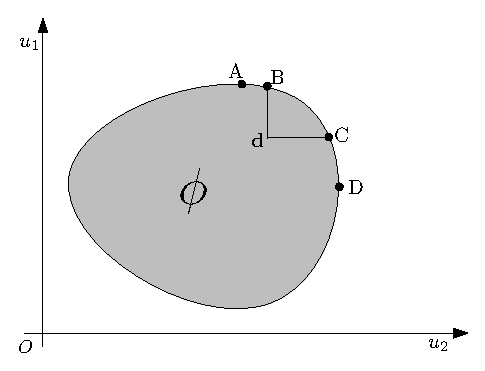
\includegraphics[width = \textwidth]{bargain_basic_concept} 
    \caption{议价概念示意图} 
    \label{fig:chap_bargain:bargain_basic_concept} 
  \end{minipage}%
\end{figure}

\subsection{纳什公理化议价博弈理论}
首先假定在一个博弈过程中存在两个参与者。
每个博弈的参与者追求使自己的效用最大化。
我们把它们分别记为$u_1$和$u_2$。
记号$\phi$表示效用向量$\mathbf{u}=(u_1, u_2)$的非空紧凸集合(Closed and bounded)。
并且,双方附加一个条件:如果博弈双方不能达成一个有约束力的协议的话,
那么,双方将会得到效用$\mathbf{b}=(d1, d2)$。
效用向量$\mathbf{d}$也被叫作原来状态(status quo)。
纳什议价博弈模型的解是这样一个函数$f$,该函数可以将集合$\phi$映射到解集上。
纳什证明,存在着唯一的一个解$\mathbf{u^*}$满足以下四条公理,解的存在性和唯一性分别由效用向量集合是紧集和凸集的性质保证。
(Nash, 1950):
\begin{itemize}
\item 公理一:弱帕累托最优性质(Weak Pareto Optimality)\\
如果$\mathbf{u} \in \phi$,而且$\mathbf{u} \ge \mathbf{u}^*$,那么可以推导得到 $\mathbf{u} = \mathbf{u}^*$
\item 公理二:对称性(Symmetry),\\
如果$d1=d2$ 并且如果$(u_1, u_2) \in \phi \Rightarrow (u_2, u_1) $, 一定有 $u_1^*= u_2^*$。
\item 公理三:规模转换不变性(Scale Transformation Covariance)\\ 
如果$\forall (a_1, a_2, b_1, b_2) \in R$,如果我们定义函数$g$是将所有向量$(u1, u2)$映射到$(u1', u2')$的函数,例如$u_i^\prime=a_iu_i+ b_i (i =1,2)$,于是我们有 $f[g(\phi), g(d)]=g[f(\phi , d)]$。
\item 公理四:无关选择的无关性(Independence of Irrelevant Alternatives) \\
如果集合$\psi \subset \phi$ ,
并且$f(\phi,d) \in \psi$,那么可得 $f(\psi,d) = f(\phi,d)$ 。
\end{itemize}

如果满足以上四个公理的情况下,
可以证明纳什议价的唯一解便是使纳什积$(u_1-d_1)(u_2-d_2)$最大化的效用向量(Nash, 1950; Osborne and Rubinstein, 1990): 
\begin{align}
\mathbf{u}^* = arg \max (u_1-d_1)(u_2-d_2)
\label{eqn:chap_nash:nash_product}
\end{align}
并满足如果 ,那么有u*≥d。对“纳什解最大化纳什积”这一定理的一个最近的证明可以参阅奥斯伯恩和鲁宾斯坦的《博弈论教程》,在这本书的最后一章中作者证明,根据四条公理所定义的纳什解,一个效用向量是纳什议价解当且仅当这一效用向量最大化纳什积(Osborne and Rubinstein, 1994)。
